\section{Overview of Approaches}
\label{sec:approach}

%\JQ{Yizhu: add here? }
%\YZ{non-neural}
In abstractive text summarization, early researchers tried non-neural abstractive summarization methods~\cite{banko-etal-2000-headline}, which used statistical models to recognize important words and sentences and then concatenate them into a final summary with or without pre-defined templates. The most direct way is to select a set of keywords from input~\cite{nenkova2005impact}, such as log-likelihood ratio test~\cite{lin2000automated}, which identified the set of words that appear in the input more often than in a background corpus. Another way is to assign weights to all words in the input, such as TF-IDF weights~\cite{berg2011jointly}. Word weights have also been estimated by supervised approaches with typical features, including word probability and location of occurrence~\cite{sipos2012large}. Some other traditional work directly focuses on predicting sentence importance, by either emphasizing select sentences that match the template of summaries or selecting the sentences in which keywords appeared near each other. Such sentences can better convey important information and be selected as a summary~\cite{celikyilmaz2010hybrid,litvak2010new}. Researchers also productively explored the relationship between word and sentence importance, and tried to estimate each in either supervised or unsupervised framework~\cite{liu2010supervised}. Since 2015, neural-based abstractive text summarization models~\cite{rush2015neural, see2017get} began to be widely developed, such as  recurrent neural network (RNN)~\cite{nallapati2016abstractive}, convolutional neural network
(CNN)~\cite{gehring2017convolutional}  and Transformer~\cite{vaswani2017attention} models. Benefiting from the semantic representation learned from large training data, neural-based methods outperform non-neural ones, especially in the aspect of fluency and semantic coherence.
\begin{figure}[t]
	\centering
	\subfigure[Sequential Modeling]{
		\begin{minipage}[t]{0.45\linewidth}
			\centering
			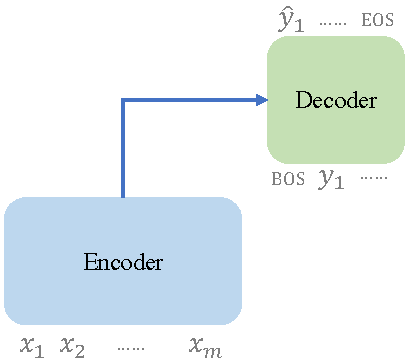
\includegraphics[scale=0.5]{fig/sequentialmodeling.pdf}
		\end{minipage}
	}
	\subfigure[Hierarchical Modeling]{
		\begin{minipage}[t]{0.45\linewidth}
			\centering
			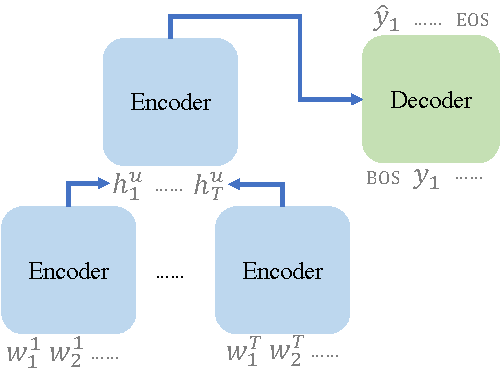
\includegraphics[scale=0.5]{fig/hierarchicalmodeling.pdf}
		\end{minipage}
	}
	\caption{Two mainstream modeling designs for encoder-decoder summarization models.}%\JQ{ are there any other methods besides neural encoder-decoder seq2seq models?}}
	\label{fig:encdec}
\end{figure}

The mainstream approaches in recent years hinge on the neural-based encoder-decoder architecture.  
In document/news summarization, 
document sentences can be concatenated into a single sequence of tokens $X=\{x_1, x_2, ..., x_m\}$ as the input to the encoder ${\rm Enc}(\cdot)$ which maps the tokens into 
contextualized hidden states $H = \{h_1, h_2, ..., h_m\}$. $m$ represents the number of input tokens. 
Besides such flat and sequential modeling, hierarchical modeling is another representative design as shown in Fig.~\ref{fig:encdec}, which is usually favored by longer dialogues. Sentences are no more concatenated but instead modeled with hierarchical encoders. The lower layer encoder projects tokens within a sentence into hidden states. Then, the higher layer encoder takes these hidden states as sentence embeddings and projects them into global hidden representations.
The decoder ${\rm Dec}(\cdot)$ takes all of the hidden states $H$ and previously generated tokens 
as input, predicting the next token step by step in an auto-regressive way. The training objective is to minimize the negative log-likelihood $L$ with the teacher-forcing strategy as follows:
\begin{equation}
	\begin{aligned}
		&H= {\rm Enc}(x_1, x_2, ..., x_m) \\
		&P(y_p|y_{<p},H) = {\rm Softmax}(W_v{\rm Dec}(BOS, y_1, y_2, ..., y_{p-1}, H))\\
		&L = -\frac{1}{n}\sum_{p=1}^n P(y_p|y_{<p}, H) 
	\end{aligned}
\end{equation}
where $W_v$ is a trainable parameter matrix mapping hidden states into a vocabulary distribution. During inference, the predicted distribution over vocabulary at step $p$ is:
\begin{equation}
		P(\hat{y}_p|\hat{y}_{<p},H) = {\rm Softmax}(W_v{\rm Dec}(BOS, \hat{y}_1, \hat{y}_2, ..., \hat{y}_{p-1}, H))
\end{equation}
%where $\hat{y}_p$ represents the generated token.
Tokens are sampled based on this distribution with generation strategies such as greedy and beam searches to produce the optimal summary. 
Greedy search selects the next token with the largest probability at each step and subsumes it into the current generation, while beam search expands each candidate generation with top-$k$ possible next tokens and preserves the $k$-best candidate generations at each step~\cite{rush2015neural}. The candidate with the highest probability is the final output.
%\JQ{add some description of "greedy search" and "beam search"} 
The decoding process starts with the beginning of a sentence (BOS) token and terminates when the end of a sentence (EOS) token is generated. 
%Basic neural architectures for encoders and decoders evolve from CNN~\cite{gehring2017convolutional} and RNN~\cite{nallapati2016abstractive} to Transformer~\cite{vaswani2017attention}.
Nowadays, pre-trained models taking advantage of the Transformer encoder-decoder architecture with sequential modelings, such as BART and Pegasus, are the state-of-the-art abstractive text summarization techniques for document summarization.


These models also work for dialogue summarization.  
For sequential modeling, utterances prefixed with corresponding speakers are simply concatenated into the 
input sequence for a dialogue, i.e. 
\begin{equation}
	X = \{x_1, x_2, ..., x_m\} = [s_1, u_1, s_2, u_2, ..., s_T, u_T]
\end{equation}
where $[\cdot]$ represents concatenation operation.
However, such a simple operation largely ignores the flexible discourse structure and topic boundaries challenges in dialogue summarization.
For hierarchical modeling, utterances $\{u^t|_{t=1}^{T}\}$ are passed into encoders separately, which sets a significant barrier for word-level cross-utterance understanding.
Besides, models pretrained with normal text are not ideal for dialogue language understanding. 
To deal with these challenges, a number of techniques have emerged. 
This survey mainly 
focuses on newly introduced techniques for adapting tested abstractive document summarization models to dialogues. 
More detailed explanations of
neural-based text summarization models and other methods please refer to
other surveys~\cite{shi2021neural,syed2021survey}.

At a high level, recent researches tackle dialogue summarization in 
three directions: %\KZ{three directions are nouns, so all three bullets 
%should be noun phrases or noun clauses.}
\begin{itemize}
\item \textbf{Injecting pre-processed features} which explicitly exploits additional features in dialogue context either by human annotators or external labeling tools as part of the input.
\item \textbf{Designing self-supervised tasks} which trains the model with auxiliary objectives besides the vanilla generation objective or individually for unsupervised summarization.
% or do manipulation on the original data with simple strategies, requiring no additional data or human annotations.
\item \textbf{Using additional data} which includes bringing training data from other related tasks or performing data augmentation based on existing training corpus.
\end{itemize}
A number of techniques have been proposed under each direction
which can be either adopted individually or combined for the targeted applications. An overall taxonomy is 
illustrated in Fig.~\ref{fig:featuretaxonomy}. The following three sections present more details, accompanied by highlights of pros and cons.
%More details about each direction are presented as follows, accompanied with a summary of pros and cons at the end of each part.

\begin{figure*}
	\centering
	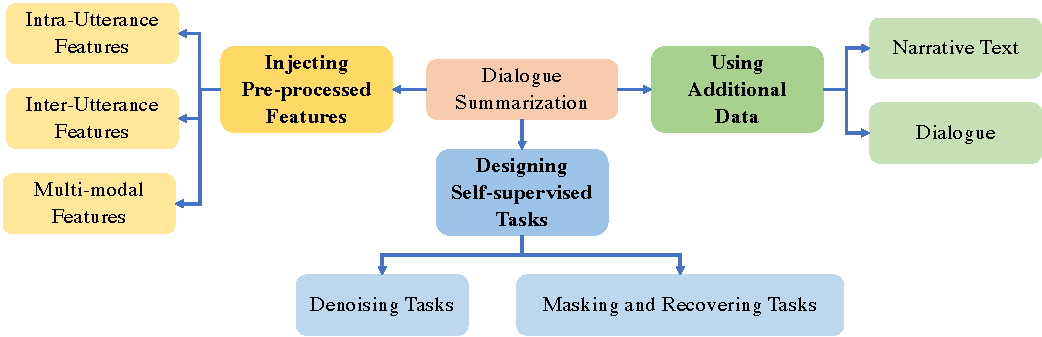
\includegraphics[scale=0.65]{fig/approaches.pdf}
	\caption{The taxonomy of dialogue summarization techniques. Methods are mainly categorized into three directions with more fine-grained sub-categories 
under each direction.}
	\label{fig:featuretaxonomy}
\end{figure*}


